\documentclass[10pt,a4paper]{article}
\usepackage[utf8]{inputenc}
\usepackage[spanish]{babel}
\usepackage{amsmath}
\usepackage{graphicx}
\usepackage{amsfonts}
\usepackage{amssymb}
\topmargin=-0.45in
\evensidemargin=0in
\oddsidemargin=0in
\textwidth=6.5in
\textheight=9.0in
\headsep=0.25in
\linespread{1.1} 
\renewcommand{\baselinestretch}{1.5}
\begin{document}
\title{Parcial 1.1}
\author{Kurth Aguilar - 20181242 }
\date{14 de agosto de 2018}
\maketitle
\section*{Solucion Problema 1}
\begin{itemize}
\item \textbf{Nodos: } \ $ \left\lbrace 1,2,3,4,5,6,7\right\rbrace $
\item \textbf{Vertices: }  
 $$
    \left\langle \left\{
        \begin{bmatrix}
            \langle 1,2 \rangle & \langle 1,3 \rangle & \langle 1,4 \rangle \\
            \langle 1,5 \rangle & \langle 1,6 \rangle & \langle 2,3 \rangle \\
            \langle 2,4 \rangle & \langle 2,5 \rangle & \langle 2,6 \rangle \\
            \langle 3,4 \rangle & \langle 3,5 \rangle & \langle 3,6 \rangle \\
            \langle 3,7 \rangle & \langle 4,7 \rangle & \langle 5,6 \rangle \\
            \langle 5,7 \rangle & \langle 6,7 \rangle &   \\
        \end{bmatrix}
    \right\} \right\rangle
$$
\item \textbf{Grafo:}
\begin{center}
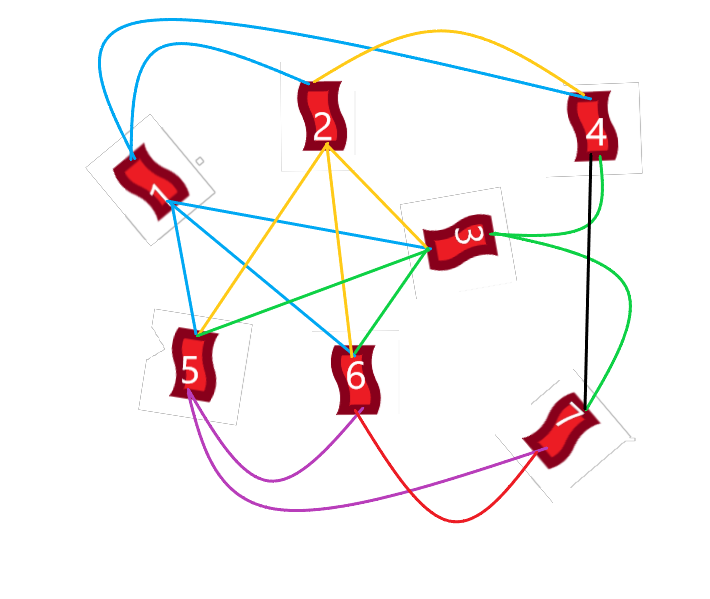
\includegraphics[width=10cm]{grafo.png}  
\end{center}
\end{itemize}
\section*{Solucion Problema 2}
\begin{center}
$ \sum_{i=1}^{n}{i}=\frac{n(n+1)}{2} $
\end{center}
\begin{itemize}
\item \textbf{Caso Base: } \ $ n = 1 $ 
\begin{center}
\
\\ $ 1 = \frac{1(1+1)}{2} $
\
\\ $ 1 = \frac{1(2)}{2}$
\
\\ $ 1 = \frac{2}{2}$
\
\\ $ 1 = 1 $
\end{center}
\item \textbf{Caso Inductivo: } $ \forall \ n$
\begin{itemize}
\item \textbf{Hipotesis Inductiva: } \ Suponiendo que el Axioma $ p5 $ de Peano se cumple, en el cual dice que una propiedad $ p(n) $ se cumple en los sucesores si el predecesor cumple con la propiedad. Entonces si suponemos que $ p(n) $ es verdadera nuestra hipotesis inductiva seria: 
\begin{center}
$ \sum_{i=1}^{n}{i}=\frac{n(n+1)}{2} $
\end{center}
\item \textbf{Sucesor: } \ $ n+1 $
\item \textbf{Demostracion: }
\begin{center}
$ \sum_{i=1}^{n}{i}= \frac{n+1(n+1+1)}{2} $
\
\\$					= \frac{n+1(n+2)}{2} $
\
\\$					= \frac{n+1 [(n+1)+1]}{2} $
\
\\\textbf{*Nota:} \ Con esta induccion o demostracion, se puede cumplir la hipotesis inductiva $ \forall n $, en la cual la propiedad $ p(n) $ se cumple. 
\end{center}
\end{itemize}
\end{itemize}

\section*{Solucion Problema 3}
\begin{center}
$ \sum_{i=1}^{n}{1} \ =1+2+3+4+\ \ldots\ +n $

\
\\ $ \sum(n)   \left\{
                        \begin{array}{ll}
                                0  & \mbox{si } n = 0 \\
                                (n-i+1) & \mbox{si } n = s(a) \ y \ i=s(b)
                        \end{array}
                \right.
$
\end{center}

\section*{Solucion Problema 4}
\begin{center}
$ a\oplus b = b\oplus a $
\end{center}
\begin{itemize}
\item \textbf{Caso Base:} 
\begin{itemize}
\item \ $ a=0$
\begin{center}
 $ 0\oplus b = b\oplus 0$
 \
 \\ $ b=b$
\end{center}
\item \ $b=0$
\begin{center}
$ a\oplus 0 = 0\oplus a $
\
\\ $ a=a$
\end{center}

\end{itemize}
\item \textbf{Caso Inductivo: } \ $ \forall \ a  $
\begin{itemize}
\item \textbf{Hipotesis Inductiva: } 
\begin{center}
$ a\oplus b = b\oplus a $
\end{center}
\item \textbf{Sucesor: } \ $s(a)$
\item \textbf{Demostracion: }
\begin{center}
\
\\$ s(a)\oplus b = b\oplus s(a) $
\
\\ $ s(a\oplus b) = b\oplus s(a)$
\
\\ $ s(a\oplus b) = s(b\oplus a)$
\
\\ \textbf{*Nota: } \ Gracias al caso base e hipotesis inductiva, se puede llegar a concluir que esto se cumple para el sucesor de cualquier numero en este caso: $ s(a)$, y su suma con otro numero: $ b $, tanto normal como viceversa, demostrando asi la comutatividad. 
\end{center}
\end{itemize}

\end{itemize}
\section*{Solucion Problema 5}
\begin{itemize}
\item \textbf{Funcion: } \ $a\geq b$
\begin{center}
$
        a\geq b =
                \left\{
                        \begin{array}{ll}
                                s(o)  & \mbox{si } b = o \\
                                o & \mbox{si } a = o \\
                                i\geq j & \mbox{si } a = s(i)\ \&\ b = s(j)
                        \end{array}
                \right.
$
\end{center}
\item \textbf{Demostrar: }
\begin{center}
$ ((n\oplus n)\geq n)= s(o)$
\end{center}
\begin{itemize}
\item \textbf{Caso Base: } \ $ n = 1 $
\begin{center}
\
\\$ ((1\oplus1)\geq 1) = s(0) $
\
\\$ ((2)\geq 1) = s(0) $
\
\\$ (2\geq 1) = s(0) $
\end{center}
\item \textbf{Caso Inductivo: } \ $ \forall \ n$
\begin{itemize}
\item \textbf{Hipotesis Inductiva: }
\begin{center}
$ ((n\oplus n)\geq n)= s(0)$
\end{center}
\item \textbf{Sucesor: } \ $ n+1 \ \ \vee \ \ s(n) $
\item \textbf{Demostracion: }
\begin{center}
\textbf{Usando s(n)}
\
\\$ ((s(n)\oplus s(n))\geq s(n)) = s(0)$
\
\\$((s(s(n\oplus n))\geq s(n)) = s(0)$
\
\\\textbf{*Nota: }\ De acuerdo con los casos expuestos de la funcion $ a\geq b$, los numeros cualquiera $ i $ y $ j $, se expresan en la funcion $ i \geq j $ cuando sus sucesores $s(i)\geq s(j)$. Entonces la funcion demostrada $ ((s(s(n\oplus n))\geq s(n))$ se cumple.
\
\\$ (s(n)\geq s(n)\circleddash s(n)) = s(o) $
\
\\$ (s(n)\geq 0) = s(0) $
\
\\\textbf{*Nota: } \ Con esto no se llega a la hipotesis inductiva, sin embargo se llega a demostrar la expresion. Porque gracias al caso $ a\geq b = s(0) \ si \ b=0$. Y en este caso $ (s(n)\geq 0) = s(0) $
\
\\
\
\\\textbf{Usando:} $ n+1 $
\
\\ $((n\oplus 1\oplus n\oplus 1)\geq n\oplus 1) = s(0)$
\
\\ $ (n\oplus 1\oplus n\oplus 1\geq n\oplus 1) = s(0)$
\
\\ $ (n\oplus 1\geq n\oplus 1\circleddash n\circleddash 1) = s(0)$
\
\\ $ (n\oplus 1\geq 0) = s(0)$
\
\\\textbf{*Nota: }\ Al igual que en el anterior no se llega a la hipotesis inductiva;sin embargo, se puede demostrar la expresion. Porque los casos de la funcion $a\geq b$, deja en explicito que la funcion es igual a $s(0)$, cuando $ b=0$, en este caso dejamos en claro que se cumple porque $ (n\oplus 1\geq 0) = s(0) $
\end{center}
\end{itemize}
\end{itemize}
\end{itemize}
\begin{center}


\end{center}

\end{document}